\documentclass{article}
\usepackage[utf8]{inputenc}
\usepackage{graphicx}
\graphicspath{}

\title{3DViewer v1.0-0}
\author{ghumbleb, mrufina, gesther}
\date{May 2022}

\begin{document}

\maketitle

\section{Introduction}
{This article is the documentation for the 3D Viewer v1.0 project, describing its main functions.}

\section{Features}
{The program supports loading a wireframe model from an .obj file (vertices and surfaces list only): you should select the file in the dialog box after pressing the button “choose file”. Supported operations with the model:}

\begin{itemize}

\item Counting the number of vertices and polygons.
\item Translation the model by a given distance in relation to the X, Y, Z axes.
\item Rotation the model by a given angle relative to its X, Y, Z axes.
\item Scale the model by a given value (as a percentage of the original size).
\item Customizing the type of projection (parallel and central).
\item Setting up the type (solid, dashed), color and thickness of the edges, display method (none, circle, square), color and size of the vertices, choosing the background color. Settings will be saved between program restarts.
\item Saving the captured (rendered) images as bmp and jpeg files.
\item Recording small screencasts by a special button - the current custom affine transformation of the loaded object into gif-animation (640x480, 10fps, 5s). After pressing the button “save gif”, the recording will start automatically.

\end{itemize}

\begin{figure}[h]
\centering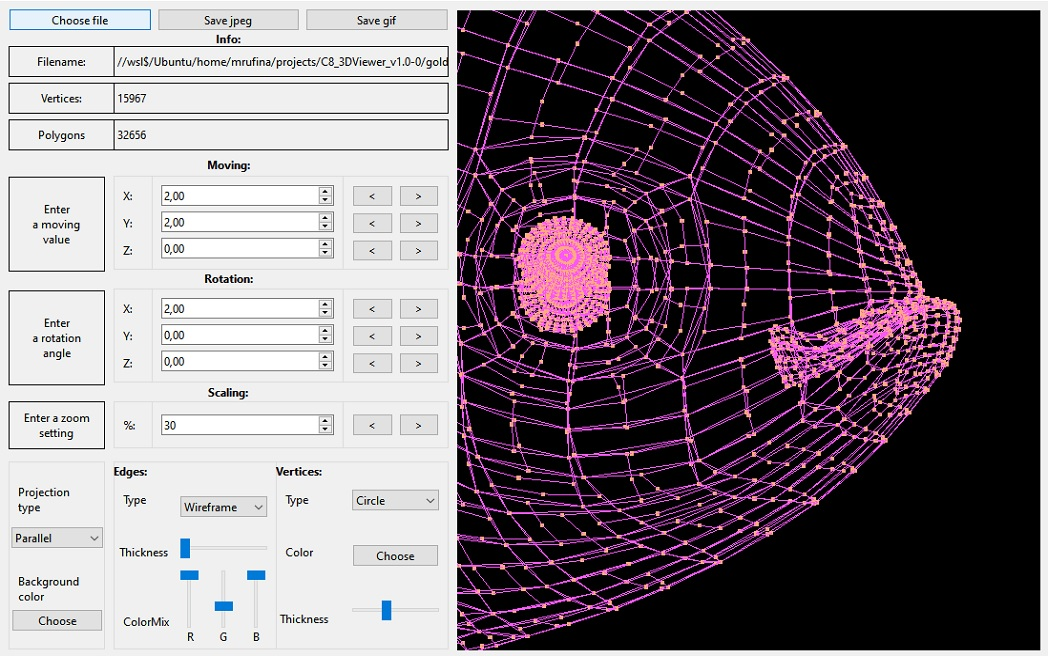
\includegraphics[scale=0.5]{example.png}
\label{fig:image}
\end{figure}

\end{document}
